\documentclass[letterpaper,landscape,9pt,fleqn]{extarticle}
%\usepackage[utf8]{inputenc}
%\usepackage[T1]{fontenc}
\usepackage{graphicx}
\usepackage{xcolor}
\usepackage{tikz}
\usepackage{url}
\usepackage{qrcode}
%\usetikzlibrary{shapes.geometric}
%\usetikzlibrary{calc}
\usepackage{array}   % for \newcolumntype macro
%\usepackage{fourier}
\usepackage{graphicx,nicefrac}
\usepackage{isomath,upgreek,xcolor,comment}
\usepackage{pdfpages}
%\usepackage{tkz-euclide}
%\usetkzobj{all}
\pagestyle{empty}
\usepackage[activate={true,nocompatibility},final,tracking=true,kerning=true,factor=1100,stretch=10,shrink=10]{microtype}
\usepackage[american]{babel}
\usepackage{centernot}
\usepackage{amstext} % for \text macro
\usepackage{array}   % for \newcolumntype macro
\newcolumntype{L}{>{$}l<{$}} % math-mode version of "l" column type

\newcommand{\dom}{\mathrm{dom}} 
\newcommand{\range}{\mathrm{range}} 
\newcommand{\zero}{\mathrm{zero}} 
\newcommand{\reals}{\mathbf{R}} 
\newcommand{\ball}{\mathrm{ball}}
\newcommand{\integers}{\mathbf{Z}} 
\newcommand{\ssep}{\mid}
\newcommand{\arcsec}{\mathrm{arcsec}}
\newcommand{\arccsc}{\mathrm{arccsc}}
\newcommand{\arccot}{\mathrm{arccot}}

\usepackage{amsmath,amssymb,textcomp}
\everymath{\displaystyle}

%\usepackage{times}
%\renewcommand\familydefault{\sfdefault}
%\usepackage{tgheros}
%\usepackage[defaultmono,scale=0.85]{droidmono}
\usepackage{fourier}
\usepackage{multicol}
\setlength{\columnseprule}{0pt}
\setlength{\columnsep}{20.0pt}

\usepackage[]{enumerate}
\usepackage{expdlist}

\newenvironment{alphalist}{
  \begin{enumerate}[(a)]
    \addtolength{\itemsep}{-1.0\itemsep}}
  {\end{enumerate}}

\usepackage{geometry}
\geometry{letterpaper,left=0.4in,right=0.4in,top=0.4in,bottom=0.4in}

%\linespread{1.3}


% custom title
\makeatletter
\renewcommand*{\maketitle}{%
\noindent
\begin{minipage}{0.4\textwidth}

\begin{tikzpicture}
\node[rectangle,rounded corners=6pt,inner sep=10pt,fill=blue!50!black,text width= 0.95\textwidth] {\color{white}\Huge \@title};
\end{tikzpicture}
\end{minipage}
\hfill
\begin{minipage}{0.55\textwidth}
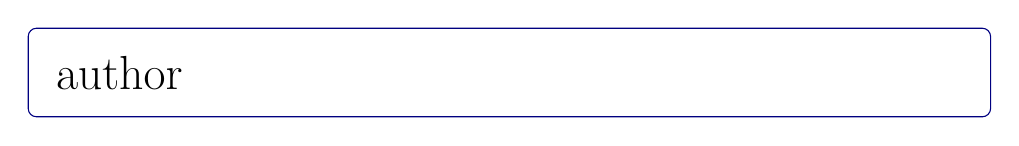
\begin{tikzpicture}
\node[rectangle,rounded corners=3pt,inner sep=10pt,draw=blue!50!black,text width= 0.95\textwidth] {\LARGE \@author};
\end{tikzpicture}
\end{minipage}
\bigskip\bigskip
}%
\makeatother

% custom section
\usepackage[explicit]{titlesec}
\newcommand*\sectionlabel{}
\titleformat{\section}
  {\gdef\sectionlabel{}
   \normalfont\sffamily\Large\bfseries\scshape}
  {\gdef\sectionlabel{\thesection\ }}{0pt}
  {
\noindent
\begin{tikzpicture}
\node[rectangle,rounded corners=3pt,inner sep=4pt,fill=blue!50!black,text width= 0.95\columnwidth] {\color{white}\sectionlabel#1};
\end{tikzpicture}
  }
\titlespacing*{\section}{0pt}{15pt}{10pt}


% custom footer
%\usepackage{fancyhdr}
%\makeatletter
%\pagestyle{fancy}
%\fancyhead{}
%\fancyfoot[C]{\footnotesize \textcopyright\ \@date\ \ \@author}
%\renewcommand{\headrulewidth}{0pt}
%\renewcommand{\footrulewidth}{0pt}
%\makeatother

\raggedbottom 
%\usepackage{tikz-3dplot}
\begin{document}

%\maketitle

\begin{multicols*}{3}

\section*{Greek Characters}
\begin{tabular}{|L | L| L|} \hline
\mbox{Name} & \mbox{Symbol} & \mbox{Typical use(s)} \\ \hline
\mathrm{alpha} & \alpha  & \mbox{ angle, constant} \\
\mathrm{beta} & \beta  & \mbox{ angle, constant}  \\ 
\mathrm{gamma} & \gamma & \mbox{angle, constant} \\
\mathrm{delta} & \delta  & \mbox{ limit definition}\\
\mathrm{epsilon} & \epsilon  \mbox{ or } \varepsilon & \mbox{limit definition} \\
\mathrm{theta}  & \theta  \mbox{ or } \vartheta &\mbox{ angle}\\ 
\mathrm{pi} & \pi \mbox{ or } \uppi & \mbox{circular constant} \\
\mathrm{phi} & \phi \mbox{ or } \varphi  & \mbox{ angle, constant} \\
\hline
\end{tabular}

\section*{Named Sets}
\begin{tabular}{|L | L |} \hline 
\mathrm{empty\,\, set} & \varnothing \\ 
\mathrm{real\,\, numbers} & \mathbf{R} \\
\mathrm{ordered \, \, pairs }  & \mathbf{R}^2 \\
\mathrm{integers } & \mathbf{Z} \\
\mathrm{positive \,\,  integers } & \mathbf{Z}_{>0} \\ 
\mathrm{positive \,\, real \,\,  numbers} & \mathbf{R}_{>0} \\
\hline
\end{tabular}

\section*{Set Symbols}
\begin{tabular}{|L | L|} \hline
\mbox{Meaning}  & \mbox{Symbol} \\ \hline
\mathrm{is \,\, a \,\, member} & \in \\
\mathrm{subset}       & \subset \\
\mathrm{intersection} & \cap \\
\mathrm{union} & \cup  \\ 
\mathrm{set \,\,  minus}  & \setminus \\ \hline
\end{tabular}
\section*{Intervals}
\begin{minipage}[c]{0.333\textwidth}
For numbers \(a\) and \(b\), we define the intervals:
\begin{align*}
 (a,b) &= \left\{x \in \reals \ssep a < x < b \right\}  \\
  [a,b) &= \{x  \in \reals  \ssep a \leq  x < b \} \\
   (a,b] &= \{x  \in \reals \ssep a <  x \leq  b \} \\
    [a,b]  &= \{x  \in \reals \ssep a \leq  x \leq  b \} \\
 %   (-\infty, a) &= \{x \mid x < a \} \\
 %   (-\infty, a] &= \{x \mid x \leq  a \} \\
 % (a, \infty)  &= \{x \mid a < x  \} \\
 %  [a, \infty)  &= \{x \mid a \leq  x  \} \\
\end{align*}  
\end{minipage}

\section*{Logic Symbols}
\begin{tabular}{|L | L|} \hline 
\mbox{Meaning}  & \mbox{Symbol} \\ \hline 
\mathrm{negation} &  \lnot   \\
\mathrm{and} &  \land  \\
\mathrm{or} &  \lor  \\
\mathrm{implies} &  \implies  \\
\mathrm{equivalent} &  \equiv \\ 
\mbox{for all} & \forall \\
\mbox{there exists} & \exists \\ \hline
\end{tabular}

\section*{Tautologies}
\begin{alignat*}{2}
    &\lnot \lnot P \equiv P \\
    &\lnot (P \land Q) \equiv \lnot P \lor \lnot Q \\
    &P \centernot \implies Q \equiv P \land \lnot Q \\
    &\lnot (\forall x \in A)(P(x)) \equiv  (\exists x \in A)(\lnot P(x)) \\
    &\lnot (\exists x \in A)(P(x)) \equiv  (\forall x \in A)(\lnot P(x)) \\
 \end{alignat*}

 \section*{Function Notation}
\begin{tabular}{|L | L|} \hline 
    \dom(F) &   \mbox{domain of function } F \\
    \range(F) &   \mbox{range of function } F \\
    C_{A} & \mbox{ set of continuous functions on set } A \\
    A \to B   & \mbox{set of functions with} A \mbox { to } B \\ \hline
\end{tabular}

\begin{comment}
\section*{Floor and ceiling}

\noindent Definitions:
\begin{align*}
    \lfloor x \rfloor = \max \{k \in \integers \mid  k \leq x \} \\
    \lceil x \rceil = \min  \{k \in \integers \mid  k \geq x \}   
\end{align*}

\noindent Properties:
\begin{align*}
   \forall(x \in \reals) (\lfloor x \rfloor \leq x) \\
   \forall(x \in \reals) (\lceil x \rceil \geq x) \\
\end{align*}
\end{comment}


  
\section*{Bounded sets}
\begin{description}%[\itemsep=0em]
    \item[bounded below] A set $A$ is bounded below provided
        \[\exists M \in \reals)(\forall x \in A)(M < x),\]

    \item[bounded above] The set $A$ is bounded above provided
        \[(\exists M \in \reals)(\forall x \in A)(x < M ). \]  
        
    \item[bounded set] A set is bounded if it is bounded below and bounded above.

\end{description}

\section*{Elementary function properties}
    \begin{description}
        \item[Increasing] \((\forall x,y \in A)(x < y \implies F(x) < F(y)) \).
        \item[Decreasing] \((\forall x,y \in A)(x < y \implies F(x) < F(y)) \).
        \item[One-to-one] \((\forall x,y \in \dom(F))(F(x) = F(y) \implies x = y) \).
        \item[Bounded above] \((\exists M \in \reals)(\forall x \in \dom(F))(F(x) < M) \).
        \item[Bounded below] \(\left (\exists M \in \reals \right) \left (\forall x \in \dom(F) \right ) \left (M < F(x) \right) \).
    \end{description}

\section*{Topology}

\begin{description}[\itemsep=1.5pt \parsep=1.5pt]
    \item[Open ball] $\ball(a, r) = \{x \in \reals \ssep -r < x-a < r \}$
  
    \item[Punctured ball] $\ball^\prime(a, r) = \ball(a, r) \setminus \{a\}$
  
    \item[Open set] A subset $A$ of $\reals$ is open provided
        \begin{equation*}  \left(\forall x \in A\right ) \left (\exists \, r \in \reals_{>0})(\ball(x,r) \subset A \right). \end{equation*} 
  
    \item[Closed set] A subset $A$ of $\reals$ is closed provided \(\reals \setminus A\) is open.
  
    \item[Limit point] A number $a$ is a limit point of a set $A$ provided
         \begin{equation*}  \forall r \in \reals_{>0})(\ball^\prime(a, r) \cap A \neq \varnothing).  \end{equation*} 

\end{description}    
\section*{Functions}   
\begin{description}
    \item[Continuous] A function $F$ is continuous at $a$ provided
    \begin{alphalist}
        \item $a \in \dom(F)$ and; 
        \item for every $\varepsilon \in \reals_{>0}$
        \item there is $\delta \in \reals_{>0}$
        \item such that for all $x \in \ball(a,\delta) \cap \dom(F)$
        \item we have $F(x) \in \ball(F(a), \epsilon)$.
    \end{alphalist}

    \item[Uniformly continuous]  A function $F$ is unformly continous on a set $A$ provided 
       \begin{alphalist}
          \item $A \subset \dom(F)$; and
          \item for every $\varepsilon \in \reals_{>0}$
          \item there is $\delta \in \reals_{>0}$
          \item such that for all $x,y  \in A \land |x-y| < \delta$
          \item we have $|F(x) - F(y)| < \epsilon$.
       \end{alphalist} 
    \item[Limit]  A function $F$ has a limit toward $a$ provided
       \begin{alphalist}
          \item $a$ is a limit point of $\dom(F)$ and;
          \item there is $L \in \reals$
          \item such that for every $\varepsilon \in \reals_{>0}$
          \item there is $\delta \in \reals_{>0}$
          \item such that for all $x \in \ball^\prime(a,\delta)$
          \item we have $F(x) \in \ball(L, \epsilon)$.
       \end{alphalist} 

    \item[Differentiable] A function $F$ is differentiable at $a$ provided
     \begin{alphalist}
    \item $a \in \dom(F)$; and
       \item there is $\phi \in \dom(F) \to \reals$
       \item such that $\phi$ is continuous at $a$ and
       \item $(\forall x \in \dom(F))(F(x) = F(a) + (x-a) \phi(x))$.
     \end{alphalist}

\end{description}
\end{multicols*}{2}
\vfill
\noindent Revised \today. Barton Willis is the author of this work. This work is
licensed under Attribution 4.0 International (CC BY 4.0) \,  \qrcode[height=0.15in]{https://creativecommons.org/licenses/by/4.0/}. For the current version of
this document, visit \, \qrcode[height=0.15in]{https://github.com/barton-willis/Math-100-200-level} 


\end{document}